% Options for packages loaded elsewhere
\PassOptionsToPackage{unicode}{hyperref}
\PassOptionsToPackage{hyphens}{url}
%
\documentclass[
]{article}
\usepackage{amsmath,amssymb}
\usepackage{lmodern}
\usepackage{ifxetex,ifluatex}
\ifnum 0\ifxetex 1\fi\ifluatex 1\fi=0 % if pdftex
  \usepackage[T1]{fontenc}
  \usepackage[utf8]{inputenc}
  \usepackage{textcomp} % provide euro and other symbols
\else % if luatex or xetex
  \usepackage{unicode-math}
  \defaultfontfeatures{Scale=MatchLowercase}
  \defaultfontfeatures[\rmfamily]{Ligatures=TeX,Scale=1}
\fi
% Use upquote if available, for straight quotes in verbatim environments
\IfFileExists{upquote.sty}{\usepackage{upquote}}{}
\IfFileExists{microtype.sty}{% use microtype if available
  \usepackage[]{microtype}
  \UseMicrotypeSet[protrusion]{basicmath} % disable protrusion for tt fonts
}{}
\makeatletter
\@ifundefined{KOMAClassName}{% if non-KOMA class
  \IfFileExists{parskip.sty}{%
    \usepackage{parskip}
  }{% else
    \setlength{\parindent}{0pt}
    \setlength{\parskip}{6pt plus 2pt minus 1pt}}
}{% if KOMA class
  \KOMAoptions{parskip=half}}
\makeatother
\usepackage{xcolor}
\IfFileExists{xurl.sty}{\usepackage{xurl}}{} % add URL line breaks if available
\IfFileExists{bookmark.sty}{\usepackage{bookmark}}{\usepackage{hyperref}}
\hypersetup{
  hidelinks,
  pdfcreator={LaTeX via pandoc}}
\urlstyle{same} % disable monospaced font for URLs
\usepackage[margin=1in]{geometry}
\usepackage{color}
\usepackage{fancyvrb}
\newcommand{\VerbBar}{|}
\newcommand{\VERB}{\Verb[commandchars=\\\{\}]}
\DefineVerbatimEnvironment{Highlighting}{Verbatim}{commandchars=\\\{\}}
% Add ',fontsize=\small' for more characters per line
\usepackage{framed}
\definecolor{shadecolor}{RGB}{248,248,248}
\newenvironment{Shaded}{\begin{snugshade}}{\end{snugshade}}
\newcommand{\AlertTok}[1]{\textcolor[rgb]{0.94,0.16,0.16}{#1}}
\newcommand{\AnnotationTok}[1]{\textcolor[rgb]{0.56,0.35,0.01}{\textbf{\textit{#1}}}}
\newcommand{\AttributeTok}[1]{\textcolor[rgb]{0.77,0.63,0.00}{#1}}
\newcommand{\BaseNTok}[1]{\textcolor[rgb]{0.00,0.00,0.81}{#1}}
\newcommand{\BuiltInTok}[1]{#1}
\newcommand{\CharTok}[1]{\textcolor[rgb]{0.31,0.60,0.02}{#1}}
\newcommand{\CommentTok}[1]{\textcolor[rgb]{0.56,0.35,0.01}{\textit{#1}}}
\newcommand{\CommentVarTok}[1]{\textcolor[rgb]{0.56,0.35,0.01}{\textbf{\textit{#1}}}}
\newcommand{\ConstantTok}[1]{\textcolor[rgb]{0.00,0.00,0.00}{#1}}
\newcommand{\ControlFlowTok}[1]{\textcolor[rgb]{0.13,0.29,0.53}{\textbf{#1}}}
\newcommand{\DataTypeTok}[1]{\textcolor[rgb]{0.13,0.29,0.53}{#1}}
\newcommand{\DecValTok}[1]{\textcolor[rgb]{0.00,0.00,0.81}{#1}}
\newcommand{\DocumentationTok}[1]{\textcolor[rgb]{0.56,0.35,0.01}{\textbf{\textit{#1}}}}
\newcommand{\ErrorTok}[1]{\textcolor[rgb]{0.64,0.00,0.00}{\textbf{#1}}}
\newcommand{\ExtensionTok}[1]{#1}
\newcommand{\FloatTok}[1]{\textcolor[rgb]{0.00,0.00,0.81}{#1}}
\newcommand{\FunctionTok}[1]{\textcolor[rgb]{0.00,0.00,0.00}{#1}}
\newcommand{\ImportTok}[1]{#1}
\newcommand{\InformationTok}[1]{\textcolor[rgb]{0.56,0.35,0.01}{\textbf{\textit{#1}}}}
\newcommand{\KeywordTok}[1]{\textcolor[rgb]{0.13,0.29,0.53}{\textbf{#1}}}
\newcommand{\NormalTok}[1]{#1}
\newcommand{\OperatorTok}[1]{\textcolor[rgb]{0.81,0.36,0.00}{\textbf{#1}}}
\newcommand{\OtherTok}[1]{\textcolor[rgb]{0.56,0.35,0.01}{#1}}
\newcommand{\PreprocessorTok}[1]{\textcolor[rgb]{0.56,0.35,0.01}{\textit{#1}}}
\newcommand{\RegionMarkerTok}[1]{#1}
\newcommand{\SpecialCharTok}[1]{\textcolor[rgb]{0.00,0.00,0.00}{#1}}
\newcommand{\SpecialStringTok}[1]{\textcolor[rgb]{0.31,0.60,0.02}{#1}}
\newcommand{\StringTok}[1]{\textcolor[rgb]{0.31,0.60,0.02}{#1}}
\newcommand{\VariableTok}[1]{\textcolor[rgb]{0.00,0.00,0.00}{#1}}
\newcommand{\VerbatimStringTok}[1]{\textcolor[rgb]{0.31,0.60,0.02}{#1}}
\newcommand{\WarningTok}[1]{\textcolor[rgb]{0.56,0.35,0.01}{\textbf{\textit{#1}}}}
\usepackage{longtable,booktabs,array}
\usepackage{calc} % for calculating minipage widths
% Correct order of tables after \paragraph or \subparagraph
\usepackage{etoolbox}
\makeatletter
\patchcmd\longtable{\par}{\if@noskipsec\mbox{}\fi\par}{}{}
\makeatother
% Allow footnotes in longtable head/foot
\IfFileExists{footnotehyper.sty}{\usepackage{footnotehyper}}{\usepackage{footnote}}
\makesavenoteenv{longtable}
\usepackage{graphicx}
\makeatletter
\def\maxwidth{\ifdim\Gin@nat@width>\linewidth\linewidth\else\Gin@nat@width\fi}
\def\maxheight{\ifdim\Gin@nat@height>\textheight\textheight\else\Gin@nat@height\fi}
\makeatother
% Scale images if necessary, so that they will not overflow the page
% margins by default, and it is still possible to overwrite the defaults
% using explicit options in \includegraphics[width, height, ...]{}
\setkeys{Gin}{width=\maxwidth,height=\maxheight,keepaspectratio}
% Set default figure placement to htbp
\makeatletter
\def\fps@figure{htbp}
\makeatother
\setlength{\emergencystretch}{3em} % prevent overfull lines
\providecommand{\tightlist}{%
  \setlength{\itemsep}{0pt}\setlength{\parskip}{0pt}}
\setcounter{secnumdepth}{5}
\usepackage{ctex}

%\usepackage{xltxtra} % XeLaTeX的一些额外符号
% 设置中文字体
%\setCJKmainfont[BoldFont={黑体},ItalicFont={楷体}]{新宋体}

% 设置边距
\usepackage{geometry}
\geometry{%
  left=2.0cm, right=2.0cm, top=3.5cm, bottom=2.5cm} 

\usepackage{amsthm,mathrsfs}
\usepackage{booktabs}
\usepackage{longtable}
\makeatletter
\def\thm@space@setup{%
  \thm@preskip=8pt plus 2pt minus 4pt
  \thm@postskip=\thm@preskip
}
\makeatother
\ifluatex
  \usepackage{selnolig}  % disable illegal ligatures
\fi
\usepackage[]{biblatex}

\author{}
\date{\vspace{-2.5em}}

\begin{document}

{
\setcounter{tocdepth}{2}
\tableofcontents
}
\hypertarget{usage}{%
\section{中文图书Bookdown模板的基本用法}\label{usage}}

\hypertarget{usage-ins}{%
\subsection{安装设置}\label{usage-ins}}

使用RStudio软件完成编辑和转换功能。
在RStudio中,安装bookdown等必要的扩展包。

本模板在安装之前是一个打包的zip文件,
在适当位置解压(例如,在\texttt{C:/myproj}下),
得到\texttt{MathJax}, \texttt{Books/Cbook}, \texttt{Books/Carticle}等子目录。
本模板在\texttt{Books/Cbook}中。

为了利用模板制作自己的中文书,
将\texttt{Books/Cbook}制作一个副本,
改成适当的子目录名,如\texttt{Books/Mybook}。

打开RStudio软件,
选选单``File - New Project - Existing Directory'',
选中\texttt{Books/Mybook}子目录,确定。
这样生成一本书对应的R project(项目)。

为了将模板内容替换成自己的内容,
可以删除文件\texttt{0101-usage.Rmd},
然后将\texttt{1001-chapter01.Rmd}制作几份副本,
如\texttt{1001-chapter01.Rmd}, \texttt{2012-chapter02.Rmd},
\texttt{3012-chapter03.Rmd}。
各章的次序将按照前面的数值的次序排列。
将每个\texttt{.Rmd}文件内的\texttt{\{\#chapter01\}}, \texttt{\{\#chapter02-sec01\}}修改能够反映章节内容的标签文本。
所有的标签都不允许重复。
参见本模板中的\texttt{0101-usage.Rmd}文件。

后面的§\ref{usage-gitbook} 和§\ref{usage-pdfbook} 给出了将当前的书转换为网页和PDF的命令,
复制粘贴这些命令到RStudio命令行可以进行转换。

\hypertarget{usage-writing}{%
\subsection{编写自己的内容}\label{usage-writing}}

\hypertarget{usage-writing-struct}{%
\subsubsection{文档结构}\label{usage-writing-struct}}

除了\texttt{index.Rmd}以外,
每个\texttt{.Rmd}文件是书的一章。
每章的第一行是用一个井号(\texttt{\#})引入的章标题。
节标题用两个井号开始,
小节标题用三个井号开始。
标题后面都有大括号内以井号开头的标签,
标签仅用英文大小写字母和减号。

\hypertarget{usage-writing-fig}{%
\subsubsection{图形自动编号}\label{usage-writing-fig}}

用R代码段生成的图形,
只要具有代码段标签,
且提供代码段选项\texttt{fig.cap="图形的说明文字"},
就可以对图形自动编号,
并且可以用如\texttt{\textbackslash{}@ref(fig:label)}的格式引用图形。
如:

\begin{Shaded}
\begin{Highlighting}[]
\FunctionTok{plot}\NormalTok{(}\DecValTok{1}\SpecialCharTok{:}\DecValTok{10}\NormalTok{, }\AttributeTok{main=}\StringTok{"程序生成的测试图形"}\NormalTok{)}
\end{Highlighting}
\end{Shaded}

\begin{figure}
\centering
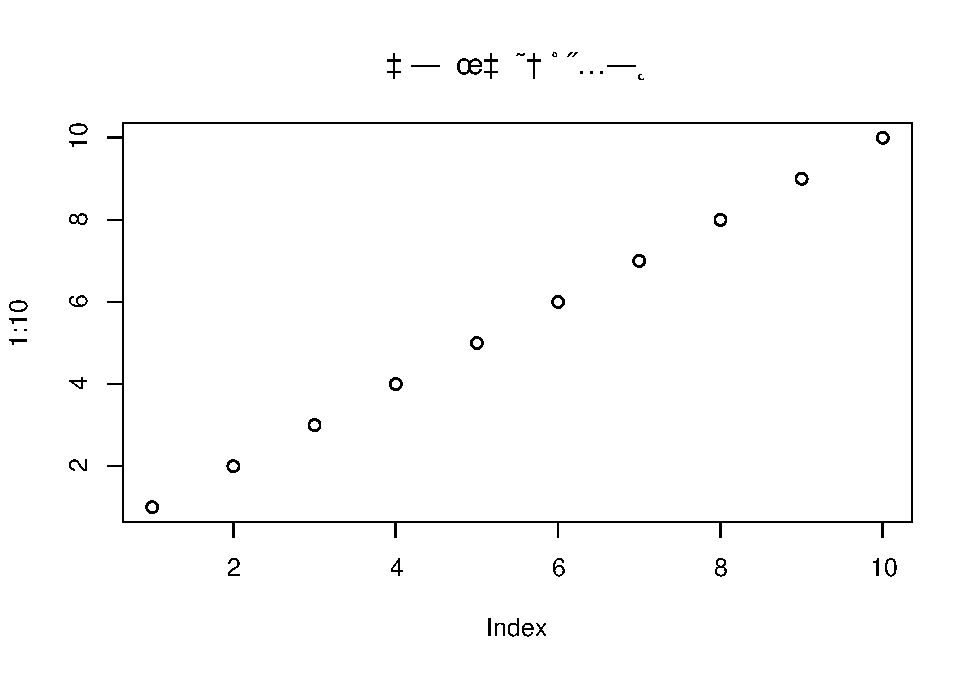
\includegraphics{0101-usage_files/figure-latex/u-w-f-ex01-1.pdf}
\caption{\label{fig:u-w-f-ex01}图形说明文字}
\end{figure}

引用如:参见图\ref{fig:u-w-f-ex01}。
引用中的\texttt{fig:}是必须的。

在通过LaTeX转换的PDF结果中,
这样图形是浮动的。

\hypertarget{usage-writing-tab}{%
\subsubsection{表格自动编号}\label{usage-writing-tab}}

用R代码\texttt{knitr::kable()}生成的表格,
只要具有代码段标签,
并且在\texttt{knitr::kable()}调用时加选项\texttt{caption="表格的说明文字"},
就可以对表格自动编号,
并且可以用如\texttt{\textbackslash{}@ref(tab:label)}的格式引用表格。
如:

\begin{Shaded}
\begin{Highlighting}[]
\NormalTok{d }\OtherTok{\textless{}{-}} \FunctionTok{data.frame}\NormalTok{(}\StringTok{"自变量"}\OtherTok{=}\DecValTok{1}\SpecialCharTok{:}\DecValTok{10}\NormalTok{, }\StringTok{"因变量"}\OtherTok{=}\NormalTok{(}\DecValTok{1}\SpecialCharTok{:}\DecValTok{10}\NormalTok{)}\SpecialCharTok{\^{}}\DecValTok{2}\NormalTok{)}
\NormalTok{knitr}\SpecialCharTok{::}\FunctionTok{kable}\NormalTok{(d, }\AttributeTok{caption=}\StringTok{"表格说明文字"}\NormalTok{)}
\end{Highlighting}
\end{Shaded}

\begin{table}

\caption{\label{tab:u-w-tab-ex01}表格说明文字}
\centering
\begin{tabular}[t]{r|r}
\hline
自变量 & 因变量\\
\hline
1 & 1\\
\hline
2 & 4\\
\hline
3 & 9\\
\hline
4 & 16\\
\hline
5 & 25\\
\hline
6 & 36\\
\hline
7 & 49\\
\hline
8 & 64\\
\hline
9 & 81\\
\hline
10 & 100\\
\hline
\end{tabular}
\end{table}

引用如:参见表\ref{tab:u-w-tab-ex01}。
引用中的\texttt{tab:}是必须的。

在通过LaTeX转换的PDF结果中,
这样的表格是浮动的。

\hypertarget{usage-writing-math}{%
\subsubsection{数学公式编号}\label{usage-writing-math}}

不需要编号的公式,
仍可以按照一般的Rmd文件中公式的做法。
需要编号的公式,
直接写在\texttt{\textbackslash{}begin\{align\}}和\texttt{\textbackslash{}end\{align\}}之间,
不需要编号的行在末尾用\texttt{\textbackslash{}nonumber}标注。
需要编号的行用\texttt{(\textbackslash{}\#eq:mylabel)}添加自定义标签,
如

\begin{align}
\Sigma =&  (\sigma_{ij})_{n\times n} \nonumber \\
=& E[(\boldsymbol{X} - \boldsymbol{\mu}) (\boldsymbol{X} - \boldsymbol{\mu})^T ] 
\label{eq:var-mat-def}
\end{align}

引用如:协方差定义见\eqref{eq:var-mat-def}。

\hypertarget{ux6587ux732eux5f15ux7528ux4e0eux6587ux732eux5217ux8868}{%
\subsubsection{文献引用与文献列表}\label{ux6587ux732eux5f15ux7528ux4e0eux6587ux732eux5217ux8868}}

将所有文献用bib格式保存为一个\texttt{.bib}文献库,
如模板中的样例文件\texttt{mybib.bib}。
可以用JabRef软件来管理这样的文献库,
许多其它软件都可以输出这样格式的文件库。

为了引用某一本书,
用如:参见\autocite{Wichmann1982:RNG}。

被引用的文献将出现在一章末尾以及全书的末尾,
对PDF输出则仅出现在全书末尾。

\hypertarget{usage-output}{%
\subsection{转换}\label{usage-output}}

\hypertarget{usage-gitbook}{%
\subsubsection{转换为网页}\label{usage-gitbook}}

用如下命令将整本书转换成一个每章为一个页面的网站,
称为gitbook格式:

\begin{Shaded}
\begin{Highlighting}[]
\NormalTok{bookdown}\SpecialCharTok{::}\FunctionTok{render\_book}\NormalTok{(}\StringTok{"index.Rmd"}\NormalTok{, }
  \AttributeTok{output\_format=}\StringTok{"bookdown::gitbook"}\NormalTok{, }\AttributeTok{encoding=}\StringTok{"UTF{-}8"}\NormalTok{)}
\end{Highlighting}
\end{Shaded}

为查看结果,
在\texttt{\_book}子目录中双击其中的\texttt{index.html}文件,
就可以在网络浏览器中查看转换的结果。
重新编译后应该点击``刷新''图标。

在章节和内容较多时,
通常不希望每次小修改之后重新编译整本书,
这时类似如下的命令可以仅编译一章,
可以节省时间,
缺点是导航目录会变得不准确。
命令如:

\begin{Shaded}
\begin{Highlighting}[]
\NormalTok{bookdown}\SpecialCharTok{::}\FunctionTok{preview\_chapter}\NormalTok{(}\StringTok{"1001{-}chapter01.Rmd"}\NormalTok{,}
  \AttributeTok{output\_format=}\StringTok{"bookdown::gitbook"}\NormalTok{, }\AttributeTok{encoding=}\StringTok{"UTF{-}8"}\NormalTok{)}
\end{Highlighting}
\end{Shaded}

单章的网页可以通过网络浏览器中的``打印''功能,
选择一个打印到PDF的打印机,
可以将单章转换成PDF格式。

\hypertarget{usage-pdfbook}{%
\subsubsection{生成PDF}\label{usage-pdfbook}}

如果想将R Markdown文件借助于LaTeX格式转换为PDF,
需要在系统中安装一个TeX编译器。
现在的rmarkdown包要求使用tinytex扩展包以及配套的\href{https://yihui.name/tinytex/}{TinyTeX软件包},
好像不再支持使用本机原有的LaTex编译系统,
如果不安装tinytex,编译为PDF格式时会出错。
TinyTeX优点是直接用R命令就可以安装,
更新也由R自动进行,不需要用户干预。
但是,安装时需要从国外网站下载许多文件,
有因为网络不畅通而安装失败的危险。

为了安装R的tinytex扩展包和单独的TinyTeX编译软件,应运行:

\begin{Shaded}
\begin{Highlighting}[]
\FunctionTok{install.packages}\NormalTok{(}\StringTok{\textquotesingle{}tinytex\textquotesingle{}}\NormalTok{)}
\NormalTok{tinytex}\SpecialCharTok{::}\FunctionTok{install\_tinytex}\NormalTok{()}
\end{Highlighting}
\end{Shaded}

安装过程需要从国外的服务器下载许多文件,
在国内的网络环境下有可能因为网络超时而失败。
如果安装成功,
TinyTeX软件包在MS Windows系统中一般会安装在 \texttt{C:\textbackslash{}Users\textbackslash{}用户名\textbackslash{}AppData\textbackslash{}Roaming\textbackslash{}MikTex}目录中,
其中``用户名''应替换成系统当前用户名。
如果需要删除TinyTeX软件包, 只要直接删除那个子目录就可以。

为了判断TinyTeX是否安装成功, 在RStudio中运行

\begin{Shaded}
\begin{Highlighting}[]
\NormalTok{tinytex}\SpecialCharTok{::}\FunctionTok{is\_tinytex}\NormalTok{()}
\end{Highlighting}
\end{Shaded}

结果应为TRUE, 出错或者结果为FALSE都说明安装不成功。
在编译\texttt{pdf\_book}时,可能会需要联网下载LaTeX所需的格式文件。

Bookdown借助操作系统中安装的LaTeX编译软件TinyTeX将整本书转换成一个PDF文件,
这需要用户对LaTeX有一定的了解,
否则一旦出错,
就完全不知道如何解决。
用户如果需要进行LaTeX定制,
可修改模板中的\texttt{preamble.tex}文件。

转换为PDF的命令如下:

\begin{Shaded}
\begin{Highlighting}[]
\NormalTok{bookdown}\SpecialCharTok{::}\FunctionTok{render\_book}\NormalTok{(}\StringTok{"index.Rmd"}\NormalTok{, }
  \AttributeTok{output\_format=}\StringTok{"bookdown::pdf\_book"}\NormalTok{, }\AttributeTok{encoding=}\StringTok{"UTF{-}8"}\NormalTok{)}
\end{Highlighting}
\end{Shaded}

在\texttt{\_book}子目录中找到\texttt{CBook.pdf}文件,
这是转换的结果。
CBook.tex是作为中间结果的LaTeX文件,
如果出错可以从这里查找错误原因。

转换PDF对于内容多的书比较耗时,
不要过于频繁地转换PDF,
在修改书的内容时,
多用\texttt{bookdown::preview\_chapter}和转换为gitbook的办法检验结果。
定期地进行转换PDF的测试。
每增加一章后都应该试着转换成PDF看有没有错误。

\hypertarget{usage-website}{%
\subsubsection{上传到网站}\label{usage-website}}

如果书里面没有数学公式,
则上传到网站就只要将\texttt{\_book}子目录整个地用ftp软件传送到自己的网站主目录下的某个子目录即可。
但是,为了支持数学公式,就需要进行如下的目录结构设置:

\begin{enumerate}
\def\labelenumi{\arabic{enumi}.}
\tightlist
\item
  设自己的网站服务器目录为\texttt{/home/abc},
  将MathJax目录上传到这个目录中。
\item
  在\texttt{/home/abc}中建立新目录\texttt{Books/Mybook}。
\item
  将\texttt{\_book}子目录上传到\texttt{/home/abc/Books/Mybook}中。
\item
  这时网站链接可能类似于\texttt{http://dept.univ.edu.cn/\textasciitilde{}abc/Books/Mybook/\_book/index.html},
  具体链接地址依赖于服务器名称与主页所在的主目录名称。
\end{enumerate}

如果有多本书,
\texttt{MathJax}仅需要上传一次。
因为\texttt{MathJax}有三万多个文件,
所以上传\texttt{MathJax}会花费很长时间。

\printbibliography

\end{document}
